\section{Removing Look-up Structures}

Now that we freely eliminate large arrays, we can focus on other
types of storage variables. The challenge we face is that the protocol of
NIPoPoWs depends on a Directed Acyclic Graph (DAG) of blocks which is constructed
using a mutable hashmap in the recommended implementation. This DAG is needed because, in the infix part of a NIPoPoW,
an adversary can skip blocks that
should normally be included in an honest proof. By using a DAG, the set of
ancestor blocks of a block is
extracted by performing a simple graph search. For the evaluation of the
predicate, the set of previously encountered \emph{ancestors} of the
tip of the longest blockchain is used.
The set of ancestors is created to avoid an adversary who presents an honest chain but
skips the block of interest.

This logic is intuitive and efficient to implement in most traditional
programming languages. However, as
our analysis demonstrates, such an implementation in Solidity is
expensive. Although Solidity supports constant-time look-up structures, native hashmaps
are only possible to hold in storage. This affects the performance of the client,
especially for large proofs.

We make a series of observations regarding the potential positions of the \emph{block of
interest} within proofs, which lead us to the construction of an architecture that
does not require maintaining a DAG, ancestors, or other complementary structures. We
consider the predicate $\pred$ to be of the form: ``does block $\boi$ exist
inside proof $\pr$?'', where $\boi$ denotes the block of interest of proof
$\pr$. Let $\es$ denote the node that performs the submission and the $\ec$
denote the node that initiates a contest.

The node $\es$ is submitting the proof $\pis$ in an attempt to convince the verifier that
the predicate $\pred$ is \emph{true}, while $\ec$ is submitting the proof $\pic$
in an attempt to convince the verifier that the predicate is \emph{false}.
We call a proof \emph{pointless} if it does not contribute to its purpose
of convincing the verifier. Namely, $\pis$ is pointless if it does contribute to convincing
the verifier of the \emph{truth} of the predicate, while $\pic$ is pointless if it
does not contribute to convincing the verifier of the \emph{falsity} of the predicate. We call
non-pointless proofs \emph{meaningful}.

\noindent \textbf{Position of block of interest.} NIPoPoWs are sets of sampled
interlinked blocks that form chains. Since proofs
$\pis$ and $\pic$ differ (otherwise the contesting proof would not be accepted),
a fork is created at
their last common ancestor $\lca$. Since $\pis$ claims the \emph{truth} of the
predicate, the block of interest $\boi$ lies at a certain
stable index~\cite{nipopows,generic-client} within $\pis$. A submission in which $\boi$ is
absent from $\pis$ is pointless, since no element
of $\pis$ satisfies $\pred$. On the contrary, if the block of
interest is included in $\pic$, then the contest is pointless.

\newcommand{\block}{\mathsf{B}}

In the NIPoPoW protocol, proof segments $\pis\{{{:}}\lca\}$ and
$\pic\{{:}\lca\}$ are merged into a single chronologically ordered chain to prevent adversaries from skipping
blocks, and the predicate is evaluated against $\pis\{{:}\lca\} \cup
\pic\{{:}\lca\}$. We observe that $\pic\{{:}\lca\}$ can be omitted during the predicate's evaluation, because no
block $\boi$ exists in $\pic\{{:}\lca\}$ that is missing from $\pis\{{:}\lca\}$
and for which the predicate holds. This is due to the fact that, in a meaningful contest, $\boi$
is not included in $\pic$. Consequently, $\pic$ is only meaningful if it forks
$\pis$ at a block prior to $\boi$.

\noindent \textbf{Minimal forks.} Given the above observation, we modify our construction
to ask the contester to only send those blocks of $\pic$ that follow the $\lca$ block.
We term this truncated chain $\pitr = \pic\{\lca{:}\}$.
In Algorithm~\ref{alg:minimal-fork}, we show how the minimal fork technique is
incorporated into our client, replacing DAG and ancestor structures.
Security is preserved by requiring that the provided $\pitr$ is a \emph{minimal fork}, namely
that it satisfies the following:

\begin{enumerate}
\item $\pis\{\lca\} = \pitr[0]$
\item $\pis\{\lca{:}\} \cap \pitr[1{:}] = \emptyset$
\end{enumerate}

The verifier checks that the above conditions are met in line~\ref{alg:minimal-fork:minimal-fork}.

In
Figure~\ref{fig:minimal-fork} we show how the performance of the client
improves. We use the same test case as in \emph{hash-and-resubmit}.
We achieve a 55\% decrease in gas
consumption. The \emph{submit} phase now costs {4{,}700{,}000} gas, and
the \emph{contest} phase costs {4{,}900{,}000} gas. Notably, after these
changes, each phase individually fits within an Ethereum block.

\renewcommand{\genesis}{\textsf{G}}

\begin{algorithm}

    \label{alg:minimal-fork}
    \caption{The \textsf{NIPoPoW} client using the minimal fork technique}

    \begin{algorithmic}[1]

    \Contract{crosschain}
    \State $\textsf{events} \gets \bot;$ $\genesis \gets \bot$
    \Function{\sf initialize}{$\genesis_{remote}$}
        \State \genesis $\gets \genesis_{remote}$
    \EndFunction
    \Function{\sf submit}{$\pis$, $e$}
        \State \textsf{require}($\pis$[0] = $\genesis$)
        \State \textsf{require}($\textsf{events$[e]$} = \bot$)
        \State \textsf{require}($\textsf{valid-interlink}(\pis)$)
        \State \textsf{events$[e]$.hash} $\gets$ \textsf{H}($\pis$)
        \State \textsf{events$[e]$.pred} $\gets$
        \textsf{evaluate-predicate}(\textsf{$\pis$}, $e$)
    \EndFunction
    \Function{\sf contest}{$\pisa$, $\pitr$, $e$, $f$}
        \Comment{$f$: fork index}
        \State \textsf{require}($\pitr$[0] = $\pisa[f]$)
        \Comment{check fork head}
        \State \textsf{require}(\textsf{events}$[e]$ $\ne$ $\bot$)
        \State \textsf{require}(\textsf{events$[e]$.hash} $=$ \textsf{H}($\pisa$))
        \State \textsf{require}(\textsf{valid-interlink}($\pitr$))
        \State \textsf{require}(\textsf{minimal-fork}($\pisa$,
        $\pitr$, $f$))
        \State \textsf{require}(\textsf{score}($\pitr$)
            $>$ \textsf{score}($\pisa[f:]$))
        \State \textsf{events$[e]$.pred} $\gets$
            \textsf{evaluate-predicate}($\pitr$, $e$)
    \EndFunction
    \Function{\sf minimal-fork}{$\pi_1$, $\pi_2$, $f$}
        \For{$p\ in\ \pi_1$}
            \If{$p \in \pi_2$}
                \State\Return false
            \EndIf
        \EndFor
    \EndFunction
    \EndContract
    \vskip8pt
    \end{algorithmic}
\end{algorithm}



\begin{figure}
    \centering
    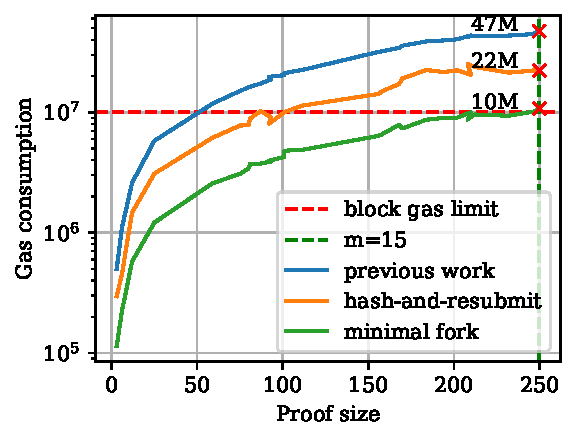
\includegraphics[width=0.7\columnwidth]{figures/minimal-fork.pdf}
    \caption{Performance improvement using minimal fork (lower is better). The
        gas consumption is decreased by approximately 55\%.}
    \label{fig:minimal-fork}
\end{figure}
